%!TEX root=../paper.tex

\chapter{Introduction}
\label{sec:intro}

Power efficiency is critical in designing and operating modern microprocessors. In the early 2000s, microprocessor designers have put low power as a first-order concern in designing digital integrated circuits~\cite{pedram2002power, rabaey2009low}, pointing out that the power density of a microprocessor could exceed that of a nuclear reactor should the clock rate continues the conventional Dennard Scaling~\cite{rabaey2002digital}, making heat dissipation a key constraint for estimating total chip power budget. More recently, as the information ecosystem has shifted towards the cloud-edge paradigm, power efficiency has been classified as a key design constraint by researchers on both ends. For datacenters, higher hardware power efficiency entails a lower total cost of ownership (TCO), which increases the profit margin of an enterprise~\cite{barroso2013datacenter}. For mobile devices, higher efficiency prolongs battery life, which improves user satisfaction~\cite{zhu2017energy}. Therefore, improving microprocessor power efficiency is an important goal for computer architecture researchers today.

While there is significant motivation to improve microprocessor power efficiency, the end of Dennard scaling and Moore's law~\cite{esmaeilzadeh2011dark,theis2017end} have made our design arsenal increasingly limited to achieve this goal. Specifically, it has become increasingly difficult to continue pushing more active cores onto the silicon real estate and relying on parallelism for improving performance while keeping power under control, as is the common practice in the past 10 years, leaving aside the difficulty of programming parallel software. As techniques are being exhausted to optimize conventional general purpose hardware, many researchers have turned to application-specific proposals, notably customized hardware design (i.e. accelerators) to reduce the power wastage of data movement and instruction decoding in general purpose chips~\cite{qadeer2015convolution}. While this approach has proven to be successful in key emerging applications domains, e.g., machine learning~\cite{chen2014diannao, jouppi2017datacenter, caulfield2016cloud, dean2018new}, its design, verification, and manufacturing costs are, however, non-negligible in the fast development cycle of today's technology world. As a result, alternative proposals with lower overhead, wider applicability, and practical power efficiency gains are still highly desirable for chip vendors as well as consumers.

This thesis seeks to improve microprocessor power efficiency by optimizing pipeline's timing margin, a long-neglected, but possibly one of the last opportunities where processor efficiency can yet be improved. The significance of this thesis topic is based on three findings. First, over 10\% power or performance gain can be achieved simply by squeezing down modern microprocessor's existing timing margin, based on real hardware measurement on production CPUs and GPUs~\cite{reddi2010voltage, leng2015safe}, which proves practical benefit can be realized by working on the excess timing margin. Second, timing margin exists for all processor architectures, from CPUs~\cite{reddi2009voltage,reddi2010voltage} to GPUs~\cite{leng2014gpuvolt, leng2015gpu, leng2015safe}, and inevitably in the upcoming accelerators. This is because all pipelined architectures need to prevent timing failure, caused by chip environment changes, such as unusual temperature, voltage noise, or process corners. Thus, some amount of margin is always required, indicating the opportunity from timing margin is pervasive. Third, to date, there is no comprehensive thesis that systematically studies a practical solution that can effectively reduce timing margin in production processors, and hence the implication for the whole computing system layers are yet to be discovered.

Specifically, this thesis focuses on studying the system-level implication of Active Timing Margin, a young technique proposed to reduce timing margin. Active timing margin uses a hardware loop to adjust chip supply voltage and frequency based on real-time monitored load environment. It has been tested rigorously on various production processors to pass load environment corner cases~\cite{lefurgy2011active,bowman201222nm,tokunaga20145,grenat20145,bowman20158,webel2015robust,vezyrtzis2018droop,fischer200590nm}. Compared with other proposals that try to trim down the timing margin~\cite{grochowski2002microarchitectural,ernst2003razor,powell2003pipeline,gupta2008decor,gupta2009event, reddi2009voltage, reddi2010voltage,miller2012vrsync,leng2015safe, papadimitriou2017harnessing}, active timing margin's low implementation overhead and execution correctness guarantee make it the more favorable design solution. Thus, understanding how active timing margin behaves and saves timing margin in the field, and trying to maximize its efficiency gain with appropriate management has practical impact for designing future computing systems.

\paragraph{Thesis Statement} Active timing margin’s full efficiency gain can only be unlocked through cross-layer management, covering hardware, platform, and software configurations. At the hardware level, we need fine-tuning core-level adaptive clocking to address process variability. At the platform level, we need power and temperature management to leverage temperature inversion. At the software level, we need application scheduling to work with voltage variation.

The rest of this chapter is organized as follows. \Sec{sec:intro:work} provides an overview of my research contributions. \Sec{sec:intro:impact} discusses the long-term practical impact of my thesis. \Sec{sec:intro:outline} outlines the rest of the dissertation and \Sec{sec:intro:prev} lists previously published materials that this dissertation draws upon.

\section{Research Contributions}
\label{sec:intro:work}

My Ph.D. research's objective is to study and optimize the active timing margin. In this pursuit, the thesis first provides an instrumental explanation over active timing margin's design and working mechanism, including one prevalent design flavor that is based on timing margin sensors that directly measures the saving room and automatically triggers voltage/frequency adjustment, and one alternative lower-cost design that uses environmental sensor such as temperature sensors to correlate the saving potential. Compared against prior proposals that optimize timing margin, the introduction highlights the significance of active timing margin as a practical and convenient solution that effectively captures the power efficiency opportunity in timing margin.

Secondly, the thesis brings the notion that to maximize active timing margin's efficiency enhancement utility, a collaborative hardware/software design that works in synergy to dynamically and safely provision timing margin is needed. This insight is based on comprehensive hardware measurement and instrumentation, which shows the proposed methods provide over 10\% measured power, or performance improvement, a highly lucrative benefit for production chips.

Thirdly, the thesis provides a complete analysis of the different system-level effects for which cross-layer management can help improve active timing margin's gain, at the author's best effort. Because timing margin in modern microprocessor pipeline is designed to combat against a wide variety of system effects, the optimization and management of active timing margin necessitate a solid understanding of all major effects that affect load environments, so that the power efficiency improvement does not hamper pipeline timing correctness. In this effort, my Ph.D. research dissects timing margin into three major components that it protects against - temperature (T), voltage (V), and process (P) variation. Although TVP variation has been thoroughly studied for static margin, their behavior are less understood in active timing margin because the technique is still new and there are not many systems available for study. I take a holistic view across system stack, spanning circuit, architecture, and application to decide for each effect what the appropriate active mechanism is to help active timing margin perform at its best.

\begin{itemize}

\item \textbf{For temperature variation:} I first propose \tistates, an active timing margin solution based on the temperature sensor, that leverages a lucrative phenomenon called \textit{temperature inversion} to reduce processor power. Then, I analyze how to help \tistates maximize its power reduction benefits, depending on the workload characteristics, the manufacturing technology node, and the chip operating temperature.

\tistates replaces the conventional static margin design where a worst-case high temperature scenario is guarded against by allocating enough margin with an active timing margin solution that tracks runtime temperature change and the resulting circuit speed variation to adjust the real-time margin dynamically. In particular, \tistates exploit the highly beneficial temperature inversion effect of CMOS transistors as technology scales down, where circuit speed accelerates significantly under higher temperature. We further show that with \tistates, runtime processor temperature can be properly managed to maximize chip power reduction, depending on the workload's activity level, and the chip's manufacturing technology.

\item \textbf{For voltage variation:}  I study a production active timing margin system, the POWER7+ multicore, where a responsive per-core hardware feedback loop is implemented that adjusts core frequency and chip supply voltage based on real-time monitored timing margin amount. Through comprehensive hardware measurements, I show that among all voltage noise components, active timing margin deals with the notorious $di/dt$ effects very effectively, which in conventional systems excess margin targeting worse-case $di/dt$ needs to be allocated. However, I find active timing margin falls short in dealing with long-term DC voltage drop, which is related to workload characteristics and chip-wide multicore activities. To maximize active timing margin's gains, we propose workload mapping management to balance compute loads on different active timing margin ``domains''. Our management points to power delivery network co-design for active timing margin. We show proper workload mapping can at least double active timing margin's power improvement.

\item \textbf{For process variation:} I take an alternative perspective and investigate how to make active timing margin automatically push the highest performance out of each core on a multicore system. To achieve this goal, I perform in-depth per-core characterization and instrumentation on POWER7+'s shipped active timing margin design. The instrumentation exposes significant performance variation across cores, which is caused by the process variation of the pipeline itself, the variation of the active timing margin hardware loop, as well as the workloads' impact on DC voltage drop, discovered in the voltage variation research aforementioned. The inter-core performance heterogeneity has previously been hidden by the multicore's default active timing margin setting, which produces
uniform frequency target across all cores. Our per-core active timing margin customization automatically brings out the core's highest speed, subject to frequency and application performance variation. To manage the performance variation of the resulting system, we propose a management scheme to improve application performance controllably. Measurement shows the proposed management boosts target application performance by over 10\%.

\end{itemize}

\begin{sidewaysfigure}
  \centering
  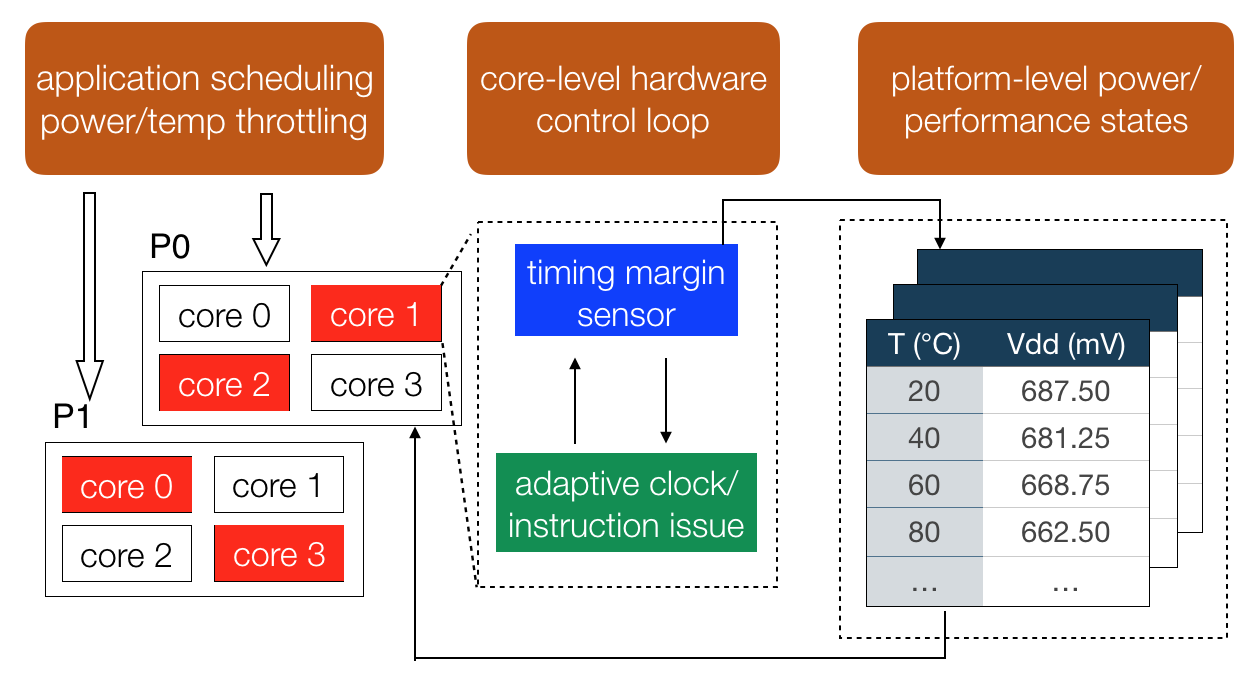
\includegraphics[trim=0 0 0 0, clip, width=\columnwidth]{graphs/intro/sys-overview.png}
  \caption{Overview of this thesis's cross-layer research on active timing margin management. We design platform-level active timing margin solution for temperature variation, characterizes state-of-the art hardware active timing margin mechanisms that deal with voltage variation, instrument core-level active timing margin fabric to expose process variation, and proposes software scheduling techniques to help these systems achieve the best power-performance gain.}
  \label{fig:framework}
\end{sidewaysfigure}

Put in the system layer context, the contribution of this thesis and the research effort I conducted to arrive at the aforementioned contributions covers circuit, architecture, and software level, illustrated by~\Fig{fig:framework}.

\textbf{At circuit and device level:} I perform hardware measurement to understand what is the granularity that timing margin sensor measures available margin, and map circuit speed/delay to temperature or voltage variation. In the \tistates proposal, the characterization of how temperature affects CMOS transistor speed, and hence available margin, is critical in building the active timing margin loop. In the voltage variation study, the dissecting of voltage noise into different components that active timing margin can, or can not deal with is built upon the understanding of how voltage affects circuit speed, using timing margin sensors.

\textbf{At architecture design level:} I propose designs that implement, or helps active timing margin perform at its best. \tistates are a set of power management states stored as tables in system firmware, which are later indexed using runtime temperature sensor readings. \tistate is essentially an evolution of classic power management states, such as P-states For voltage variation, the analysis we make points to an alternative power delivery network design which is separated into different domains, with each domain covering a few cores to minimize per-domain DC voltage drop and maximize active timing margin's voltage reduction capability.

\textbf{At system software and application level:} I propose application mapping and throttling technique on multicore systems to manage a microprocessor's DC voltage drop, with the goal of reducing total processor power or enhancing target application performance. The software solution serves as a complement to the hardware-only active timing margin mechanism and is proven by measurement to double the power reduction, or performance improvement gain.

\section{Long-term Impact}
\label{sec:intro:impact}

As Dennard scaling and Moore's law approaching their end, and general-purpose architectures becoming ripe, it is vital that the research contributed to enhancing processor power efficiency have practical long-term impact, or they perish. The long-term impact of my thesis lies in three fundamental aspects:

First, my thesis on optimizing microprocessor timing margin has wide applicability in the semiconductor industry. It is not dependent upon one processor architecture and does not affect and interfaces between hardware and software. \tistates was carried out on the GPU of an APU System-on-Chip (SoC), while the study on optimizing timing margin for voltage and process variation was conducted on a multicore platform. In principle, any processor architecture can benefit from the insights and proposals in this dissertation, including accelerators, if ultra power efficiency is desired. 

Second, the active timing margin technique has seen proven commercial success by the time this dissertation is made. When I first initiated this research topic five years ago, only a few processors are designed with active timing margin, mostly for experimenting and testing purpose~\cite{lefurgy2011active, bowman201222nm}. Today, the latest high-end chips almost all adopt this technique to squeeze out the last bit of power efficiency from silicon~\cite{tokunaga20145,grenat20145,bowman20158,webel2015robust,vezyrtzis2018droop} because of its effectiveness and convenience for implementation. In this context, our work that tries to optimize active timing margin provides a free extra mile for chip vendors to increase the efficiency gain, proving its long-term impact.

Thirdly, all results and analysis presented in this thesis are acquired from solid, real hardware measurement. Acquiring and interpreting the type of data in this thesis is very difficult, which involves a deep study of a hardware platform's internals. The measurement data not only proves the improvements and insights we made can sustain future work's tests, but also provide trustworthy, valuable guidance for other researchers who need a reference. Thus, this dissertation's impact is of high practicality.


\section{Dissertation Organization}
\label{sec:intro:outline}

The rest of my dissertation is organized as follows. 
\Sec{sec:background} introduces the basics of pipeline timing margin, prior proposals that try to optimize it, and why active timing margin is the design choice today. 
\Sec{sec:temperature}, \Sec{sec:voltage}, and \Sec{sec:process} describe the proposed active timing margin management schemes for temperature, voltage, and process variation, respectively. The work in these chapters are built upon solid characterization and analysis using hardware measurement, and the proposed work cross architecture and software design. \Sec{sec:conc} provides a retrospective and prospective view of my dissertation work. The retrospective part summarizes the principles distilled from this work on building a maximally efficient active timing margin system; the prospective part suggests next steps for generalizing our work into massive industry adoption.

\section{Previously Published Material}
\label{sec:intro:prev}

This dissertation contains materials that are previously published in peer-reviewed conferences and journals:

\textbf{\Sec{sec:background}}. The introduction on timing margin sensors, environmental sensors, and the control loop for active timing margin is a collection of the part of the materials published in the following papers: \textit{\tistates: Processor Power Management in the Temperature Inversion Region}. Yazhou Zu, Wei Huang, Indrani Paul and Vijay Janapa Reddi. In International Symposium on Microarchitecture (MICRO), 2016~\cite{zu2016tistate}; \textit{Adaptive guardband scheduling to improve system-level efficiency of the POWER7+}. Yazhou Zu, Charles R. Lefurgy, Jingwen Leng, Matthew Halpern, Michael S. Floyd and Vijay Janapa Reddi. In International Symposium on Microarchitecture (MICRO), 2015~\cite{zu2015adaptive}; \textit{Active Timing Margin Management for Maximizing Multi-Core Efficiency on an IBM POWER7+ Server}. Yazhou Zu, Daniel Richins, Charles R. Lefurgy and Vijay Janapa Reddi. In International Symposium on High Performance Computer Architecture (HPCA)~\cite{zu2019atm}.

\textbf{\Sec{sec:temperature}}. The design and management of active timing margin for temperature variation are based on the following paper: \textit{\tistates: Processor Power Management in the Temperature Inversion Region}. Yazhou Zu, Wei Huang, Indrani Paul and Vijay Janapa Reddi. In International Symposium on Microarchitecture (MICRO), 2016~\cite{zu2016tistate}. A modified version of this paper is also published in IEEE's annual Top Picks selection: \textit{\tistates: Power Management in Active Timing Margin Processors}. Yazhou Zu, Wei Huang, Indrani Paul and Vijay Janapa Reddi. In IEEE Micro, June 2017, 37(3):106-114~\cite{zu2017ti}. I am the lead author of these papers, and I was responsible for proposing the idea, experimenting with it and evaluating the final results.

\textbf{\Sec{sec:voltage}}. The characterization of on-chip voltage noise, as well as its active timing margin management for power saving is based on the following paper: \textit{Adaptive guardband scheduling to improve system-level efficiency of the POWER7+}. Yazhou Zu, Charles R. Lefurgy, Jingwen Leng, Matthew Halpern, Michael S. Floyd and Vijay Janapa Reddi. In International Symposium on Microarchitecture (MICRO), 2015~\cite{zu2015adaptive}. I am the lead author of this paper. I conducted all the comprehensive characterization experiments, proposed the idea to improve microprocessor power saving, and performed the associated evaluation.

\textbf{\Sec{sec:process}}. The work on active timing margin management for multicore process variation is is based on the following paper: \textit{Active Timing Margin Management for Maximizing Multi-Core Efficiency on an IBM POWER7+ Server}. Yazhou Zu, Daniel Richins, Charles R. Lefurgy and Vijay Janapa Reddi. In International Symposium on High Performance Computer Architecture (HPCA), 2019~\cite{zu2019atm}. I am the lead author of this paper. I proposed the idea, performed the design space exploration, and conducted all performance improvement evaluation.

\textbf{Other publications}: During the length of my Ph.D., I've also worked on other related topics and made joint publications in GPU voltage analysis, Integrated Voltage Regulator analysis, etc. The co-authored papers are \textit{GPUVolt: Modeling and characterizing voltage noise in GPU architectures}. Jingwen Leng, Yazhou Zu, Minsoo Rhu, Meeta Gupta and Vijay Janapa Reddi. In International Symposium on Low Power Electronics and Design (ISLPED), 2014~\cite{leng2014gpuvolt}; \textit{GPU voltage noise: Characterization and hierarchical smoothing of spatial and temporal voltage noise interference in GPU architectures}. Jingwen Leng, Yazhou Zu and Vijay Janapa Reddi. In International Symposium on High Performance Computer Architecture (HPCA), 2015~\cite{leng2015gpu}; \textit{Ivory: Early-stage design space exploration tool for integrated voltage regulators}. An Zou, Jingwen Leng, Yazhou Zu, Tao Tong, Vijay Janapa Reddi, David Brooks, Gu-Yeon Wei and Xuan Zhang. In Design Automation Conference (DAC) 2017~\cite{zou2017ivory}; \textit{Efficient and reliable power delivery in voltage-stacked manycore system with hybrid charge-recycling regulators}. An Zou, Jingwen Leng, Xin He, Yazhou Zu, Vijay Janapa Reddi and Xuan Zhang. In Design Automation Conference (DAC) 2018~\cite{zou2018efficient}; \textit{Voltage-Stacked GPUs: A Control Theory Driven Cross-Layer Solution for Practical Voltage Stacking in GPUs}. An Zou, Jingwen Leng, Xin He, Yazhou Zu, Christopher D. Gill, Vijay Janapa Reddi and Xuan Zhang. In International Symposium on Microarchitecture (MICRO), 2018~\cite{an2018control}. As co-authors of these papers, I help brainstorm ideas, carry out necessary experiments with the lead author, and refine the writing of these papers.